\chapter{VEGAS}\label{chap:vegas}

\section{Overview}\label{sec:vegas_overview}

The \glsfirst{VEGAS} is an \gls{FPGA} based spectrometer that can be
used with any receiver except \gls{MUSTANG}. It consists of eight independent
spectrometers (banks) that can be used simultaneously. Eight-bit samplers and
polyphase filter banks are used to digitize and generate the spectra --
together they provide superior spectral dynamic range and \gls{RFI}
resistance. For details on the design of VEGAS, please consult
\htmladdnormallink
{http://www.gb.nrao.edu/vegas/report/URSI2011.pdf}
{http://www.gb.nrao.edu/vegas/report/URSI2011.pdf}.

Observers can use between one and eight dual-polarization spectrometers
(or \dq{banks}) at the same time (see Fig.~\ref{fig:vegasconfig}. Each bank
within VEGAS can be configured with a different spectral resolution,
bandwidth, and number of spectral windows (subbands). However, the integration
time, switching period, and the frequency switch {\bf must} be the same for
all banks. The resolution and bandwidth of all subbands in a single
VEGAS bank must be identical, but the center frequencies may be set
independently (within limits).

Although the individual banks could be arranged to cover 10~GHz
of total bandwidth, the maximum bandwidth is typically limited to 4-6~GHz
by filters in the \gls{GBT} \gls{IFsys} (see your project friend
for more information). All banks have the same switching signal
(i.e., same switching period, same itegration time, same frequency switch),
which is controlled by spectrometer bank \dq{A}. Each bank can be configured
in one of the 29 modes listed in Table~\ref{tab:vegas_modes}.

\begin{itemize}[leftmargin=*]
\item {\bf Modes 1-19} provide a single subband per bank.  Modes 1--3 have the
following constraints on useable bandwidth:
\begin{itemize}
\item {\bf Modes 1-2}: Have a useable bandwidth of 1250~MHz within the baseband
bandwidth of 1500~MHz.  The useable baseband frequency range is 150--1400~MHz.
\item {\bf Mode 3}: Has a useable bandwidth of 800~MHz within the baseband
bandwidth of 1080~MHz.  The useable baseband frequency range is 150--950~MHz.
\end{itemize}
\item {\bf Modes 20-29} provide up to eight subbands per bank.  All subbands
must have equal bandwidths and be placed within the total bandwidth processed
by that bank:
\begin{itemize}
\item {\bf Modes 20-24}: Have a useable bandwidth of 1250~MHz within the baseband
bandwidth of 1500~MHz.  The useable baseband frequency range is 150--1400~MHz.
\item {\bf Modes 25-29}: Have a useable bandwidth of 800~MHz within the baseband
bandwidth of 1080~MHz.  The useable baseband frequency range is 150--950~MHz.
\end{itemize}
\end{itemize}

Each mode provides the polarization products XX, YY, and optionally XY,YX
necessary for observations of polarized emission without requiring a reduction
in the number of channels or sampling speed. VEGAS can also record only a single
polarization for single-polarization receivers.





\begin{table}[!h]
\begin{center}
\begin{footnotesize}
\caption[VEGAS Modes]
{VEGAS Modes supported by each of the 8 \gls{VEGAS} spectrometers.
\label{tab:vegas_modes}}
\begin{tabular}{ c c r d r r}
\toprule
\multicolumn{1}{c}{Mode} & Bandwidth & \multicolumn{1}{c}{Channels} & \multicolumn{1}{c}{Spectral}&
\multicolumn{1}{c}{Minimum}      & \multicolumn{1}{c}{Max data rate$^a$}     \\
                         & (MHz)     &                              & \multicolumn{1}{c}{resolution}&
\multicolumn{1}{c}{int. time$^b$}& \multicolumn{1}{c}{at minimum int.}            \\
                         &           &                              & \multicolumn{1}{c}{(kHz)}&
\multicolumn{1}{c}{(ms)}         & \multicolumn{1}{c}{time (MBs$^{-1}$) } \\
\midrule
\multicolumn{6}{c}{ Single Sub-band modes$^c$} \\
\midrule
1    & 1500  & 1024 & \multicolumn{1}{c}{1465} & 1 & 32       \\
2    & 1500  & 16384 & \multicolumn{1}{c}{92} & 2 & 187     \\
3    & 1080  & 16384 & \multicolumn{1}{c}{66} & 4 & 130     \\
4    & 187.5 & 32768 &    5.7 & 11 & 52  \\
5    & 187.5 & 65536 &    2.9 & 22 & 52  \\
6    & 187.5 & 131072 &    1.4 & 35 & 69 \\
7    & 100    & 32768 &    3.1 & 12 & 51    \\
8    & 100 & 65536 &    1.5 & 25 & 51    \\
9    & 100 & 131072 &    0.8 & 40 & 69   \\
10   &  23.44 & 32768 &    0.7 & 16 & 93 \\
11   &  23.44 & 65536 &    0.4 & 33 & 93     \\
12   &  23.44 & 131072 &    0.2 & 72 & 75    \\
13   &  23.44 & 262144 &    0.1 & 134 & 93   \\
14   &  23.44 & 524288 &    0.04 & 246 & 125 \\
15   &  11.72 & 32768 &    0.4 & 27 & 93     \\
16   &  11.72 & 65536 &    0.2 & 55 & 93     \\
17   &  11.72 & 131072 &    0.1 & 123 & 62   \\
18   &  11.72 & 262144 &    0.04 & 223 & 93  \\
19   &  11.72 & 524288 &    0.02 & 447 & 93  \\
\midrule
\multicolumn{6}{c}{ 8 Sub-band modes$^c$} \\
\midrule
20  &  23.44 & 4096 &    5.7 & 6 & 12 \\
21  &  23.44 & 8192 &    2.9 & 12 & 12 \\
22  &  23.44 & 16384 &    1.4 & 35 & 8 \\
23  &  23.44 & 32768 &    0.7 & 51 & 12 \\
24  &  23.44 & 65536 &    0.4 & 97 & 13 \\
25  &  16.9 & 4096 &    4.1 & 8 & 9 \\
26  &  16.9 & 8192 &    2.1 & 17 & 9 \\
27  &  16.9 & 16384 &    1.0 & 47 & 6 \\
28  &  16.9 & 32768 &    0.51 & 69 & 9 \\
29  &  16.9 & 65536 &    0.26 & 132 & 10 \\

\bottomrule
\end{tabular}
\end{footnotesize}
\begin{footnotesize}
\begin{itemize}[itemsep=0pt]
\item[$^a$] Maximum data rate is calculated for recording full polarization
and all channels at the minimum integration period for one spectrometer.
Each spectral value is represented by 4 bytes.
\item[$^b$] The integration per switching state shoule be $\ge$ the minimum
integration. For example, if an observation uses 2 switching states, then
the minimum integration will be 2 times the value listed in the table.
\item[$^c$] For modes 20$\rightarrow$24 the subbands can be placed within
the baseband bandwidth of 1500~MHz (see note $d$) and for modes 25$\rightarrow$29
the subbands can be placed within 1000~MHz.
\item[$^d$] The usable frequency range for baseband bandwidth of 1500~MHz
(modes 1 \& 2, also for modes 20$\rightarrow$24) is 150--1400~MHz and for bandwidth
of 1000~MHz (mode 3, also for modes 25$\rightarrow$29) it is 150--950~MHz.
\end{itemize}
\end{footnotesize}
\end{center}
\end{table}

\section{Data Rates}\label{sec:vegas_data_rates}

The data rate for an individual bank can be calculated using

\begin{align}
\text{Data Rate (GB/hr)} = 1.34\times10^{-5} \cdot\dfrac{
n_{channels}\times n_{spw}\times n_{stokes}\times n_{states}}{t_{int}\text{(seconds)}}
\end{align}

where $n_{channels}$ is the number of channels per spectral window,
$n_{spw}$ is the number of spectral windows, $n_{stokes}$ is the
number of stokes parameters (2 for dual polarization, 4 for full
polarization), $n_{states}$ is the number of switching states (4 for
frequency switching and 2 for total power), and $t_{int}$ is the
integration time. The total data rate for a project can be calculated
by adding the data rates for each bank together.


\begin{figure}[!h]
\begin{center}
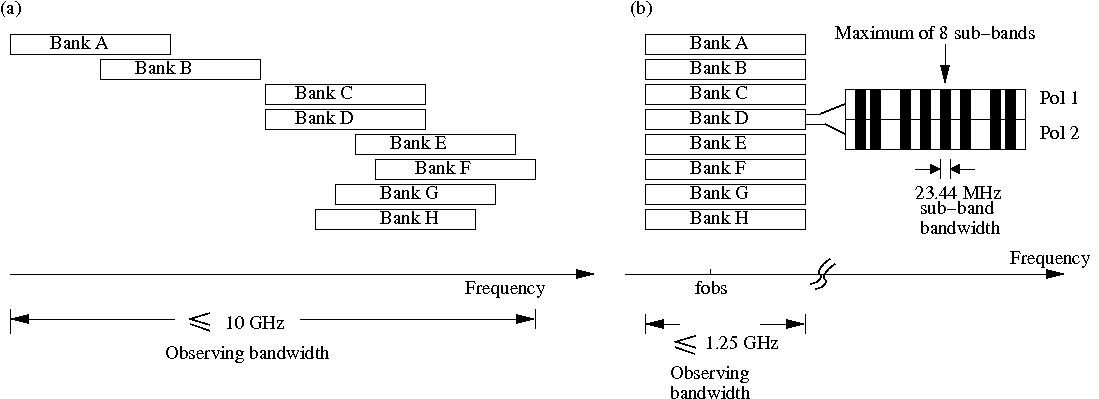
\includegraphics[width=\linewidth]{vegas8spec.jpg}
\caption[VEGAS setups]{Examples of two basic VEGAS setups. Since each bank
  can be configured independently, these setups can be mixed and
  matched with the restriction that all banks have the same switching signal.
  (a) {\em Wide band, single beam, dual polarization observations.}
  The 8 banks can be tuned to a different frequencies where each bank
  produces a single spectral window.
  (b) {\em Narrow band, multiple beam, dual polarization mode}.  Each bank can provide
  a maximum of 8 spectral windows (subbands).}
\label{fig:vegasconfig} 
\end{center}
\end{figure}

\newpage

\vspace{-1cm}

\section{IF Configuration}\label{sec:vegas_if}
The \gls{GBT} \gls{IFsys} introduces some constraints on routing signals
from the receivers to VEGAS.

\begin{itemize}[itemsep=0pt]
\item Single beam receivers or multi-beam receiver that has been configured to use
a single beam may be routed to any or all of the VEGAS banks A$\rightarrow$H.
No spectral resolution is gained with VEGAS by only using one beam of a multi-beam
receiver.
\item Dual-beam configurations allow each beam to be routed to a maximum of
4 VEGAS banks.
\item When using 3--4 beams, each beam may be routed to up to a maximum of
2 VEGAS banks.
\item When using more than 5 beams, each beam may only be routed to a
single VEGAS bank.
\item When using all 7 beams of the \gls{KFPA}, each beam may be routed to a single
VEGAS bank with an optional second copy of beam 1 being routed to the remaining
VEGAS bank. This is known as the \dq{7+1} mode of the \gls{KFPA}
\end{itemize}

\section{Blanking}\label{sec:vegas_blanking}
While the observing system is switching between states (such as switching the 
\glspl{noiseDiode} on or off, switching frequencies, running doppler updates, etc...)
the collected data is not valid, and thus must be 'blanked' by VEGAS. VEGAS 
allows the user to switch states frequently enough that the required blanking 
time can become a non-negligible percentage of the total observing time. For
efficient observing, It is important to choose switching periods that are 
long enough for the total amount of blanking to be negligible. The amount of 
blanking per switching signal is dependent on the VEGAS mode used. Conservative
values are shown in Tables~\ref{tab:blanking_cal} and~\ref{tab:blanking_nocal}
for values with the \gls{noiseDiode} turned either on or off. For a more thorough
description of the appropriate switching periods for a given amount of blanking,
and more accurate estimates of the minimum switching periods we refer the
interested reader to
\htmladdnormallink
{http://library.nrao.edu/public/memos/gbt/GBT\_288.pdf}
{http://library.nrao.edu/public/memos/gbt/GBT_288.pdf}

\newpage

\begin{table}[!h]
\begin{small}
\begin{center}
\caption[Minimum recommended switching periods for VEGAS observations
using a noise diode.]
{Minimum recommended switching periods (swper) with VEGAS for
observations that use a noise diode.
\label{tab:blanking_cal}}
\vspace{2.5mm}
\begin{tabular}{cdddd}
\toprule
 & \multicolumn{1}{c}{ {\bf{\Gls{tpower}}} ({\tt tp}) } & \multicolumn{3}{c}{{\bf\Gls{fsw}}$^a$ ({\tt sp})}\\
\cmidrule(lr){2-2}\cmidrule(lr){3-5}
  & \myalign{c}{Nominal$^b$}  & \myalign{c}{Nominal$^c$} & \myalign{c}{$\nu_{min}$$^d$(GHz)} & \myalign{c}{Mapping$^e$} \\
{\bf Mode}     &  \myalign{c}{swper (sec)} & \myalign{c}{swper (sec)} & \myalign{c}{swper=1.52 sec} & \myalign{c}{swper (sec)}  \\
\midrule
1  &0.01   & 0.4    & 115.0  & 0.4   \\
2  &0.028  & 0.4    & 115.0  & 0.4  \\
3  &0.04   & 0.4    & 115.0  & 0.4   \\
4  &0.028  & 0.4    & 115.0  & 0.4  \\
5  &0.0559 & 0.4    & 115.0  & 0.4 \\
6  &0.1118 & 0.4318 & 115.0  & 1.52   \\
7  &0.0524 & 0.4    & 115.0  & 0.4 \\
8  &0.1049 & 0.4249 & 115.0  & 1.52   \\
9  &0.2097 & 0.5297 & 59.6   & 1.52   \\
10 &0.2237 & 0.5437 & 54.4   & 1.52   \\
11 &0.4474 & 0.8948 & 16.5   & 1.52   \\
12 &0.8948 & 1.7896 &        & 1.7896 \\
13 &1.7896 & 3.5791 &        & 3.5791 \\
14 &3.5791 & 7.1583 &        & 7.1583 \\
15 &0.4474 & 0.8948 & 16.5   & 1.52   \\
16 &0.8948 & 1.7896 &        & 1.7896 \\
17 &1.7896 & 3.5791 &        & 3.5791 \\
18 &3.5791 & 7.1583 &        & 7.1583 \\
19 &7.5383 & 14.3166 &       & 14.3166 \\ %100 MHz switch
20 &0.028  & 0.4    & 115.0  & 0.4 \\
21 &0.0559 & 0.4    & 115.0  & 0.4 \\
22 &0.1118 & 0.4318 & 115.0  & 1.52 \\
23 &0.2237 & 0.5437 & 54.4 & 1.52 \\
24 &0.4474 & 0.8948 & 16.5 & 1.52 \\
25 &0.0388 & 0.4    & 115.0  & 0.4 \\
26 &0.0777 & 0.4    & 115.0  & 1.52 \\
27 &0.1553 & 0.4753 & 89.7 & 1.52 \\
28 &0.3107 & 0.6307 & 33.8 & 1.52 \\
29 &0.6214 & 1.2428 & 8.6  & 1.52 \\

\bottomrule
\end{tabular}
\end{center}
\end{small}
\end{table}
\begin{footnotesize}
\begin{itemize}[itemsep=0pt]
\item[$^a$] When frequency switching, switching periods must always be $>$0.4 seconds
due to the settling time of the \gls{LOone}.
\item[$^b$] Recommended minimum switching period ({\tt swper}) for \gls{tpower}
observations with \glspl{noiseDiode} ({\tt swtype='tp'}). These values will yield less
than 10\% blanking overall.
\item[$^c$] Recommended minimum switching period for \gls{fsw} observations with
\glspl{noiseDiode} ({\tt swtype='sp'}). These values will yield less than
10\% blanking in the first state of the switching cycle as well as less than
10\% blanking overall.
\item[$^d$] The minimum recommended switching period is 1.52 seconds {\bf when Doppler tracking}
frequencies above $\nu_{min}$.
\item[$^e$] Recommended minimum switching period ({\tt swper}) for {\bf Doppler-tracked}, \gls{fsw}
observations with \glspl{noiseDiode} ({\tt swtype='sp'}). These values will yield less than 10\%
blanking in the first state of the switching cycle as well as less than 10\% blanking overall.
This switching period will result in less than 10\% of the data being blanked. These values
assume that the maps are sampled at twice Nyquist in the scanning direction and that there are four
integrations per switching period.
{\bf when Doppler tracking}.
\end{itemize}
\end{footnotesize}
\newpage

\begin{table}[!h]
\begin{small}
\begin{center}
\caption[Minimum recommended switching periods for VEGAS
observations not using a noise diode.]
{Minimum recommended switching periods (swper) with VEGAS for
observations that do not use a noise diode.
\label{tab:blanking_nocal}}
\vspace{2.5mm}
\begin{tabular}{cdddcd}
\toprule
 & \multicolumn{2}{c}{ {\bf{\Gls{tpower}}} ({\tt tp\_nocal}) } & \multicolumn{3}{c}{{\bf\Gls{fsw}}$^a$ ({\tt sp\_nocal})}\\
\cmidrule(lr){2-3}\cmidrule(lr){4-6}
  & \myalign{c}{Nominal$^b$}  & \myalign{c}{Mapping$^c$} & \myalign{c}{Nominal$^d$} & \myalign{c}{$\nu_{min}$$^e$(GHz)} & \myalign{c}{Mapping$^f$} \\
{\bf Mode}     &  \myalign{c}{swper (sec)} & \myalign{c}{swper (sec) }& \myalign{c}{swper (sec)} & \myalign{c}{swper=0.76 sec} & \myalign{c}{swper (sec)}  \\
\midrule
1  & 0.0005 & 0.001  & 0.4    & 115.0  & 0.4 \\
2  & 0.0014 & 0.0028 & 0.4    & 115.0  & 0.4 \\
3  & 0.002  & 0.004  & 0.4    & 115.0  & 0.4 \\
4  & 0.01   & 0.0114 & 0.4    & 115.0  & 0.4 \\
5  & 0.0199 & 0.0227 & 0.4    & 115.0  & 0.4 \\
6  & 0.0301 & 0.0357 & 0.4    & 115.0  & 0.76 \\
7  & 0.0102 & 0.0128 & 0.4    & 115.0  & 0.4 \\
8  & 0.0203 & 0.0256 & 0.4    & 115.0  & 0.76 \\
9  & 0.0301 & 0.0406 & 0.4    & 115.0  & 0.76 \\
10 & 0.0056 & 0.0168 & 0.4    & 115.0  & 0.76 \\
11 & 0.0112 & 0.0336 & 0.4474 & 33.1   & 0.76 \\
12 & 0.028  & 0.0727 & 0.8948 &        & 0.8948 \\
13 & 0.0447 & 0.1342 & 1.7896 &        & 1.7896 \\
14 & 0.0671 & 0.2461 & 3.5791 &        & 3.5791 \\
15 & 0.0056 & 0.028  & 0.4474 & 33.1   & 0.76 \\
16 & 0.0112 & 0.0559 & 0.8948 &        & 0.8948  \\
17 & 0.0336 & 0.123  & 1.7896 &        & 1.7896 \\
18 & 0.0447 & 0.2237 & 3.5791 &        & 3.5791 \\
19 & \myalign{c}{0.0895 or$^g$ 0.38}   & 0.4474 & 7.1583 & & 7.1583 \\ % @10.3
20 & 0.0051 & 0.0065 & 0.4    &  115.0 & 0.4 \\
21 & 0.0101 & 0.0129 & 0.4    &  115.0 & 0.4 \\
22 & 0.0301 & 0.0357 & 0.4    & 115.0  & 0.76 \\
23 & 0.0405 & 0.0517 & 0.4    & 115.0  & 0.76 \\
24 & 0.0755 & 0.0979 & 0.4474 & 33.1   & 0.76 \\
25 & 0.007  & 0.009  & 0.4    &  115.0 & 0.4 \\
26 & 0.0141 & 0.018  & 0.4    &  115.0 & 0.76 \\
27 & 0.0398 & 0.0476 & 0.4    & 115.0  & 0.76 \\
28 & 0.0544 & 0.0699 & 0.4    & 68.6   & 0.76 \\
29 & 0.101  & 0.132  & 0.6214 & 17.1   & 0.76 \\

\bottomrule %Doppler tracking swper=0.76 above v_min
\end{tabular}
\end{center}
\end{small}
\end{table}
\begin{footnotesize}
\begin{itemize}[itemsep=0pt]
\item[$^a$] When frequency switching, switching periods must always be $>$0.4 seconds
due to the settling time of the \gls{LOone}.
\item[$^b$] Recommended minimum switching period ({\tt swper}) for \gls{tpower}
observations that do not use \glspl{noiseDiode} ({\tt swtype='tp\_nocal'}).
This value is equivalent to the hardware exposure value for VEGAS.
\item[$^c$] Recommended minimum switching period ({\tt swper}) for
\gls{tpower} \gls{OTF} mapping observations that do not use \glspl{noiseDiode}
({\tt swtype='tp\_nocal'}) {\bf when Doppler Tracking}. These values will yield less
than 10\% blanking overall and assume that the maps are sampled at twice Nyquist in
the scanning direction and that there are four integrations per switching period.
\item[$^d$] Recommended minimum switching period for \gls{fsw} observations that do not
make use of \glspl{noiseDiode} ({\tt swtype='sp\_nocal'}). These values will yield less than
10\% blanking in the first state of the switching cycle as well as less than 10\% blanking overall.
\item[$^e$] The minimum recommended switching period is 0.76 seconds {\bf when Doppler tracking}
frequencies above $\nu_{min}$.
\item[$^f$] Recommended minimum switching period ({\tt swper}) for {\bf Doppler-tracked}, \gls{fsw}
\gls{OTF} mapping observations without \glspl{noiseDiode} ({\tt swtype='sp\_nocal'}). These values
will yield less than 10\% blanking in the first state of the switching cycle as well as less
than 10\% blanking overall.  This switching period will result in less than 10\% of the
data being blanked. These values assume that the maps are sampled at twice Nyquist in the
scanning direction and that there are four integrations per switching period.
\item[$^g$] For mode 19 this value is 0.0895/0.38 seconds for observations below/above 10.3~GHz
{\bf when Doppler tracking}.
\end{itemize}
\end{footnotesize}
\newpage





\section{Monitoring VEGAS observations}\label{sec:vegas_monitoring}

The Spectral Line tab in the \gls{Astrid} Data Display (See
\S~\ref{sec:spectral_data_display}) is not fully capable of displaying
VEGAS observations in real time (it will display passbands at the end of a
scan, and may be used in offline mode). Rather, there are four monitoring tools
that are useful with VEGAS:

\begin{itemize}
\item the VEGAS Data Display at \htmladdnormallink
{https://vegasdisplay.gb.nrao.edu/}
{https://vegasdisplay.gb.nrao.edu/} (See \S~\ref{sec:vegasdisplay}).
\item the VEGAS \gls{CLEO} screen (See \S~\ref{sec:vegas_cleo}).
\item VEGASDM -- the VEGAS Data Monitor (See \S~\ref{sec:vegasdm}).
\item vegas\_status -- the VEGAS shared memory display
      (See \S~\ref{sec:vegas_status}).
\end{itemize}

The first three items are generally useful while observing with VEGAS and are
described in \S~\ref{sec:vegas_monitoring_tools}, while {\tt vegas\_status} is for
specialized problem diagnosis and is described in
Appendix~\ref{appendix:vegas_reference}.


\section{The Online Filler and Filling VEGAS data using SDFITS}
\label{sec:vegas_sdfits}
VEGAS writes \dq{Engineering} FITS files. Once a scan is over, the
\dq{Filler} reads these files, combines the data with metadata from the
Antenna and other FITS files, and produces a single-dish (SDFITS) file.
This can be done automatically, by the on-line filler, or manually by the
Observer. Due to the significantly higher data rate, and some other features
of VEGAS, the filling process requires some oversight by the user.

\subsection{The Online Filler}\label{sec:vegas_filler}
The online filler will make every attempt to fill the SDFITS file automatically.
In this case, a file will be produced in:

{\tt /home/sdfits/$<$project$>$}

and GBTIDL can connect to it automatically using the \dq{online}, or
\dq{offline, $<$project$>$} commands. There are some caveats, however.

\begin{itemize}[leftmargin=*]
\item Because of the way VEGAS writes it's data, the filler cannot start
filling until the scan has finished. For immediate inspection of data, 
Observers are urged to use the real-time display
(see \S~\ref{sec:vegasdisplay}).
\item For \dq{large} scans, the filler could potentially fall behind the
data acquisition process. To avoid this, the filler will skip scans that
it cannot keep up with. The rule is:

\begin{verbatim}
If (integration time / total number of spectra per integration) < 0.00278s
   skip the scan
Except if (integration length >= 0.9s) it will be filled
\end{verbatim}
\end{itemize}


The total number of spectra per integration is the total across all banks. So, 
for example, 2 banks, 8 subbands, 2 polarizions and  4 switching states (e.g.
frequency switching with calibration) will produce 2*8*2*4 = 128 spectra, and
so if the integration time is $<$ 0.356s the online filler will not fill 
that data. The 0.9s limit is because for that integration time the online 
filler can almost keep up even in the worst case, and interscan latencies, 
pauses for pointing and focus scans, and so on will nromally allow it time 
to catch up. The online filler prints a summary
in {\tt /home/sdfits/$<$project$>$/$<$project$>$.log} indicating what scans were
filled, had problems and were skipped, and if any data was skipped because
the data rate was too fast.

The decision on whether to fill or not is made independently for each bank.
For cases where the integration time is close to the limit it's possible that 
some banks might be filled while others are not filled for the same scan 
if the number of subbands or the number of polarizations vary across the banks.  
The summary log file will indicate when this happens.

If observers are concerned about the interpolation across the center channel 
(see \S~\ref{sec:vegas_spike}) they can turn that off in sdfits by using the
\dq{-nointerp} option.

 
\subsection{Filling Offline}\label{sec:vegas_sdfits_offline}
You may wish to (re-) fill your data offline. In this case, you make use
the SDFITS filler program in the standard manner.  Note however, that the
actual VEGAS data is stored to a high-speed (\dq{lustre} file system.  For
a current list of lustre client machines please see\\  \htmladdnormallink
{http://www.gb.nrao.edu/pubcomputing/public.shtml}
{http://www.gb.nrao.edu/pubcomputing/public.shtml} 

\noindent If you try to fill data without being logged into a lustre client,
the filler will fail with the error message:

\begin{verbatim}
VEGAS data expected but not found, this workstation is not a lustre client.
For a list of public lustre client workstations see: 
http://www.gb.nrao.edu/pubcomputing/public.shtml
\end{verbatim}

\noindent --In this case, ssh to a lustre client (using the domain {\tt .gb.nrao.edu}),
and fill your data there.

Filling using sdfits directly (instead of the output online sdfits) 
might also be useful if there are a lot of spectra to be processed in \gls{GBTIDL} 
simply because it improves the response times in \gls{GBTIDL} if there are not 
as many spectra to search through.  So if there's a convenient way to 
divide up the scans, then this sort of syntax works (sdfits -help for more details):

\begin{verbatim}
sdfits -backends=vegas -scans=<scan-list> <PROJECT_SESSION> <OUTPUT_PREFIX>
\end{verbatim}

\begin{itemize}[leftmargin=*,itemsep=0pt]
\item {\tt scan-list} is a list of comma separated scans to fill using colons to
denote ranges e.g.,\\ {\tt -scans=1,4:6,10:} would fill scans 1,4,5,6 and all
scans from 10 onwards.
\item {\tt $<$PROJECT\_SESSION$>$} is what you'd expect, e.g. \dq{AGBT14A\_252\_04}.
\item {\tt $<$OUTPUT\_PREFIX$>$} is the leading part of the output directory name,
e.g. {\tt scan5to25} would result in a directory named {\tt scan5to25.raw.vegas}
\end{itemize}

\section{Instrumental Features and their Cure}\label{sec:vegas_features}

The architecture of the VEGAS hardware, specifically the architecture
of the \gls{ADC}, results in some characteristic features in the VEGAS spectrum. 
Specifically, these are:

\begin{itemize}[itemsep=0pt]
\item a strong spurious single-channel wide spike at the exact center of 
the \gls{ADC} passband, - the so-called \dq{center spike}.
\item weak single-channel wide spurs at various locations in the 
bandpass - the 32 spurs.
\end{itemize}

\subsection{The Spike}
\label{sec:vegas_spike}
The center spike is caused by the \gls{FPGA} clock. By default, the
center spike  is interpolated over by the SDFITS filler by taking the
mean of the adjacent channel on either sided of the spike. The center spike
is also interpolated-over by the real-time spectrum display. We have chosen
to interpolate over this spike as it is omnipresent, and can cause problems 
for data reduction (such as system temperature calculations).
If you are concerned about this process, you may shift your line from the 
center of the passband using the deltafreq keyword in your astrid script.

\subsection{The Spurs}
When attempting to search for \gls{RFI} with VEGAS by running a high-pass
filter through the data, significantly more spikes/spurs were found than
naively expected. These spurs could be found in the same bins in relatively
\gls{RFI} free wavelengths, such as \gls{Qband}. The spurs appear at the same
location (in bin space) for a given mode and have relatively stable
amplitudes. These faint spurs are not always directly visible in the data,
but became clear when high-pass filtered, as shown in
Figure~\ref{fig:vegas_spurs}. After significant testing, it was determined
that these spurs are below the spurious-free dynamic range of -60dBc
specified by the manufacturer, and cannot be fully removed.
In overly simplistic terms, the spurs are caused by the leaking of the 
\gls{FPGA} clock into the four interleaved \glspl{ADC}.  For further
information see \S~\ref{sec:vegas_spurs_detailed}.

\begin{figure}[!h]
\begin{center}
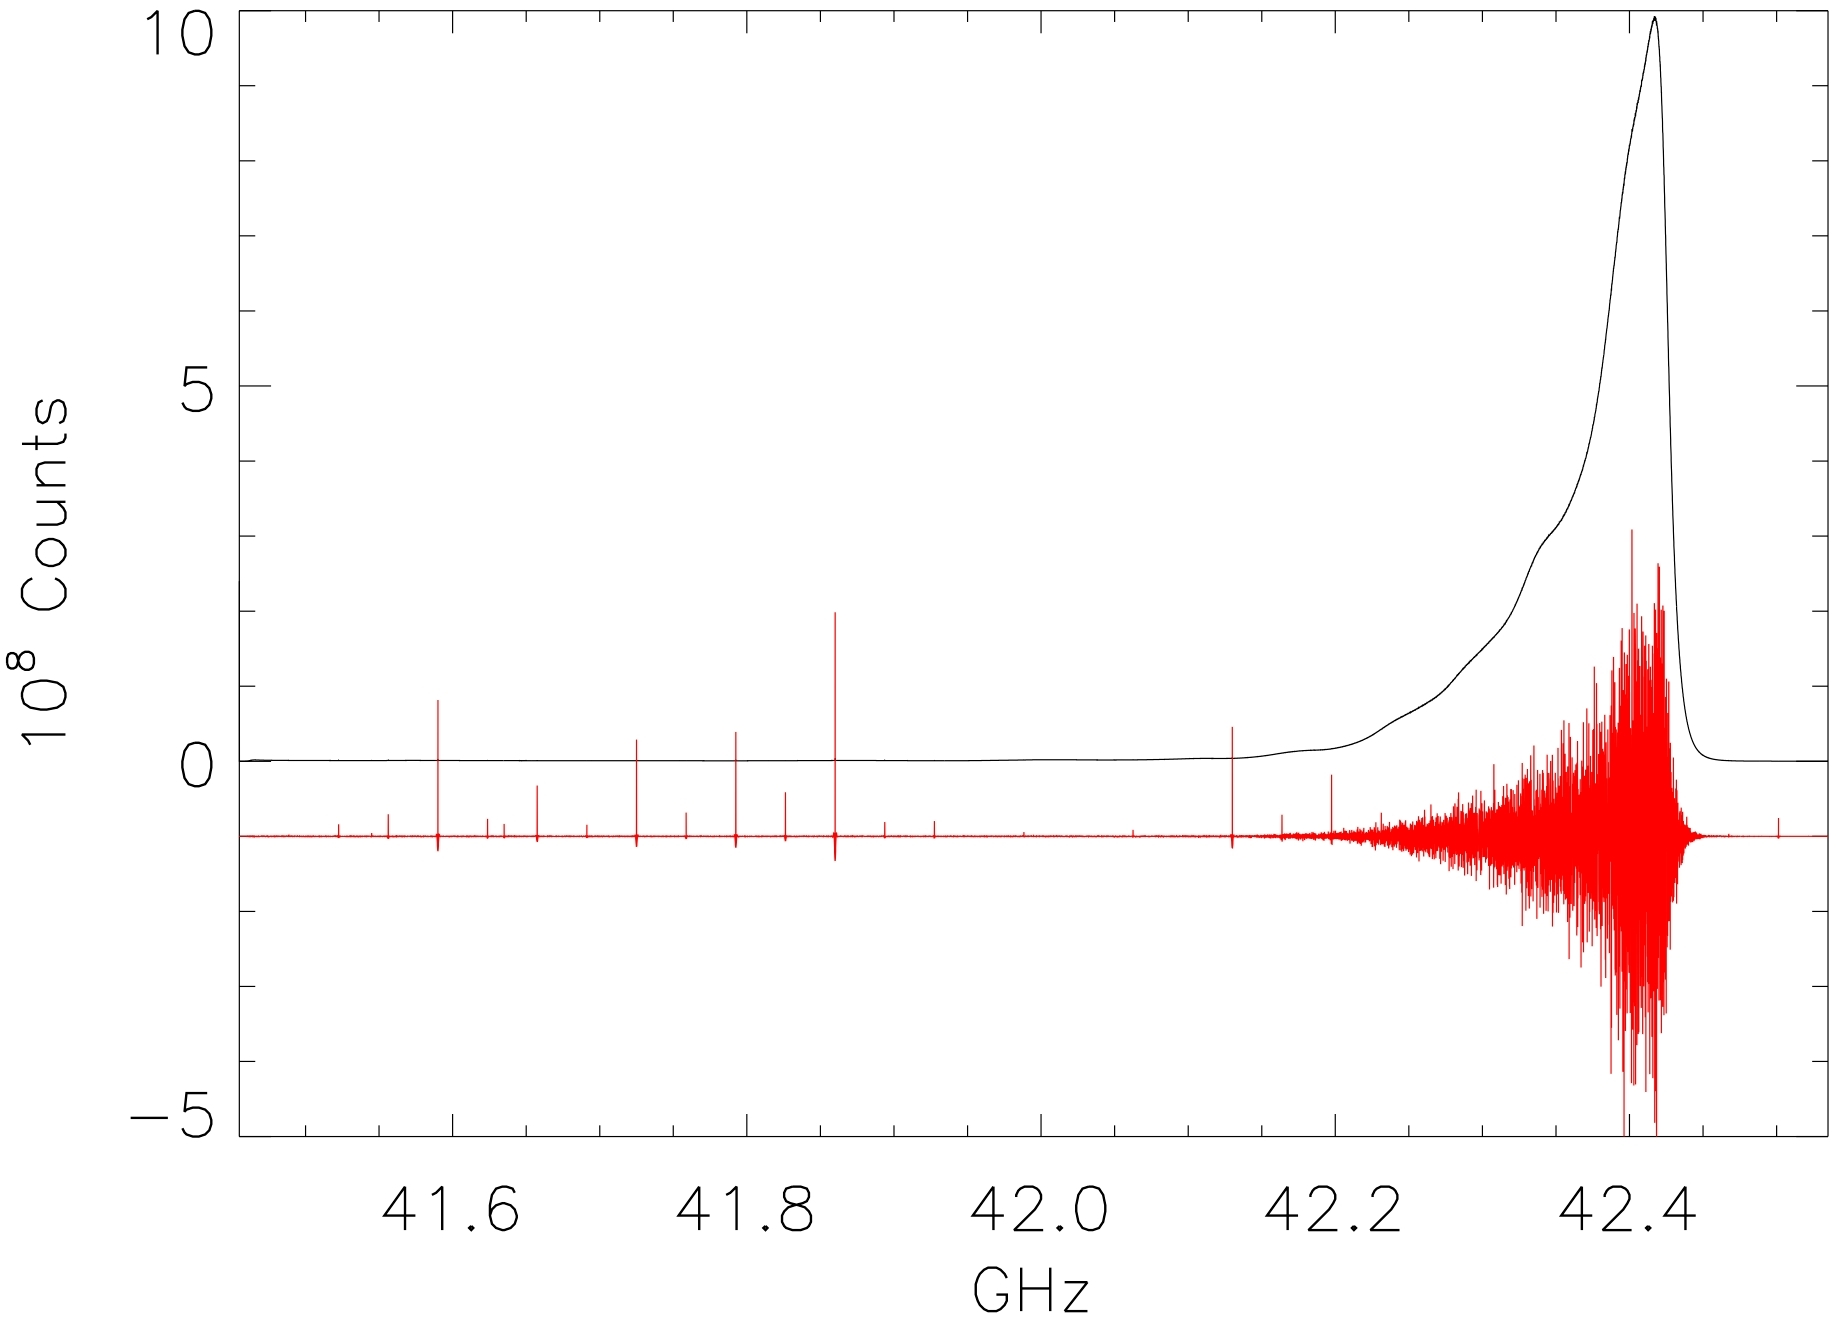
\includegraphics[width=0.8\linewidth]{raw_with_digital_filt.jpg}
\caption[VEGAS spurs]{Spectra of a noise source centered near 42.4 GHz (black). 
A high pass filtered version of the data (offset by -1 and scaled by a 
factor of 100 for visibility) is shown in red, showing the spurs.}
\label{fig:vegas_spurs}
\end{center}
\end{figure}

These spurs are relatively stable and will remain constant 
(for a given mode) and the magnitude of the spurs is relatively constant. 
These features are also quite small by most standards (Spurious Free 
Dynamic Range no more than -60dBc), but nevertheless can be problematic 
when looking for faint narrow features. The stability of these features 
allows them to be removed by standard data practices (such as position 
and/or frequency switching), but they are an added noise source which can 
bleed through to the final product. Due to the limited and often 
negligible effect of these spurs, we do not automatically interpolate across 
them, but let the user decide how to handle those channels.

\newpage

\section{Known Bugs and Features}\label{sec:vegas_bugs}
\subsection{vegasdisplay is not updating, or is running very slowly}
This occasionally happens. The cure is to ask the Operator to restart the
display:

\begin{verbatim}
TaskMaster gbtdata stop 15
TaskMaster gbtdata start 15
\end{verbatim}

\subsection{Data is not filling}

The online filler checks for project changes when it is not actively filling
a scan. This means that if the previous project was a VEGAS one and it ended
on a long scan, the filler may still be filling that project when the VEGAS
scan has finished in your project. If you suspect that this is the case, the
only solution is to ask the Operator to restart the online filler task.

--- All data can still be accessed in \gls{GBTIDL} by running SDFITS offline
(see \S~\ref{sec:vegas_sdfits_offline}).

\subsection{There is a \dq{square wave} and/or divot in my VEGASDM display}

The samples which are taken to produce the VEGASDM total power display
run asynchronously to the switching signals. Hence, the sampling may occur
during the \dq{Cal on} phase at one point in time, and then drift into
the \dq{Cal off} phase sometime later. This may produce an apparent square
wave in the VEGASDM output, with an amplitued of a few tenths of a dB, and
a period of seconds.

Similarly, it is possible for the VEGASDM data to be acquired when the \gls{LO}
is updating (e.g. during a Doppler track). These data are blanked in the
true VEGAS spectral data acquisition, but may cause drop-outs in the
VEGASDM samples.




%\begin{figure}[h!]
%\begin{center}
%\begin{latexonly}
%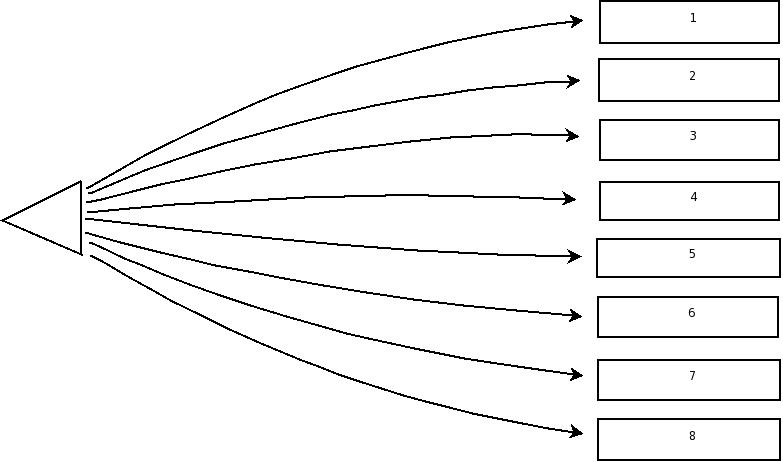
\includegraphics[width=4in]{vegas-single-beam.jpg}
%\end{latexonly}
%\begin{htmlonly}
%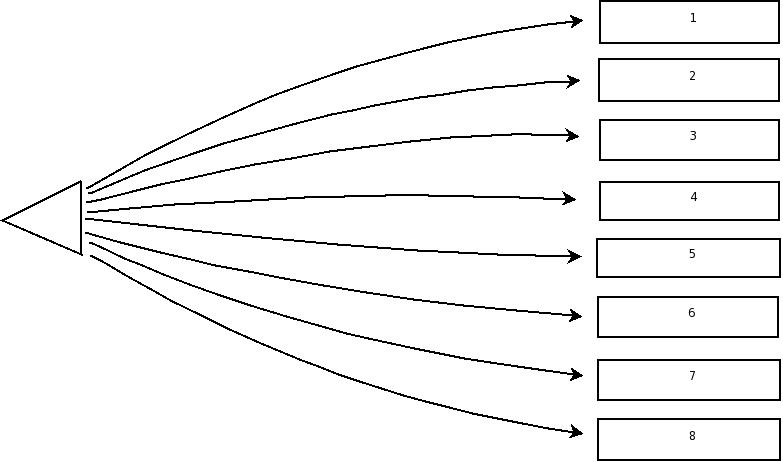
\includegraphics{vegas-single-beam.jpg}
%\end{htmlonly}
%\end{center}
%\caption[Single Beam Receiver to VEGAS Mapping.]{A graphic
%demonstration of how single beam receivers and beam 1 of the KFPA can
%be routed to the VEGAS banks.  The routing can be to 1, 2, 3,
%4, 5, 6, 7 or 8 different VEGAS banks.  This routing is not
%applicable to a single beam of a dual beam receiver.}
%\label{fig:vegassingle}
%\end{figure}

%\begin{figure}[h!]
%\begin{center}
%\begin{latexonly}
%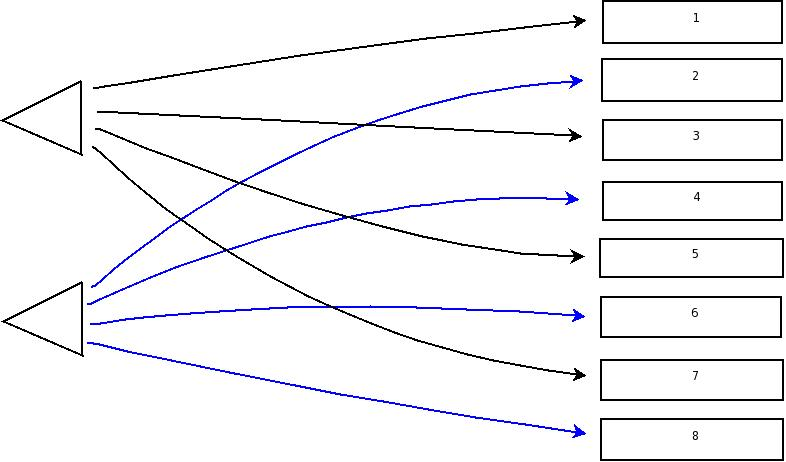
\includegraphics[width=4in]{vegas-dual-beam.jpg}
%\end{latexonly}
%\begin{htmlonly}
%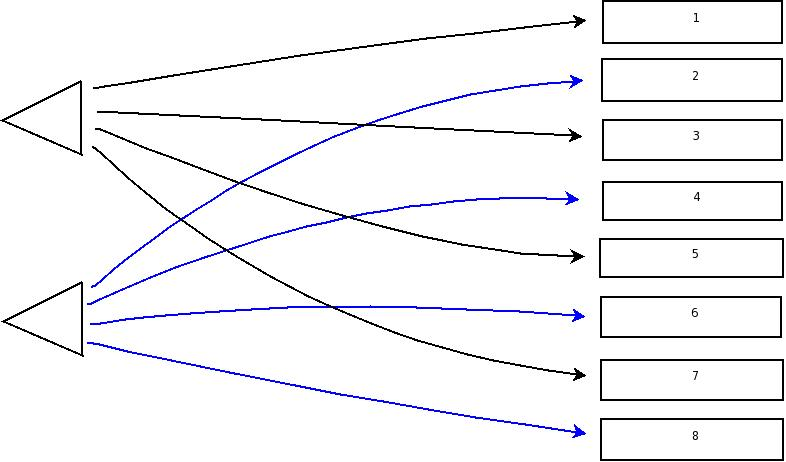
\includegraphics{vegas-dual-beam.jpg}
%\end{htmlonly}
%\end{center}
%\caption[Dual Beam Receiver to VEGAS Mapping.]{A graphic demonstration
%of how dual beam receivers, including two beams of the KFPA, can be
%routed to the VEGAS banks.  Each beam can be routed to 1, 2,
%3, or 4 different VEGAS banks. }
%\label{fig:vegasdual}
%\end{figure}


%\begin{figure}[h!]
%\begin{center}
%\begin{latexonly}
%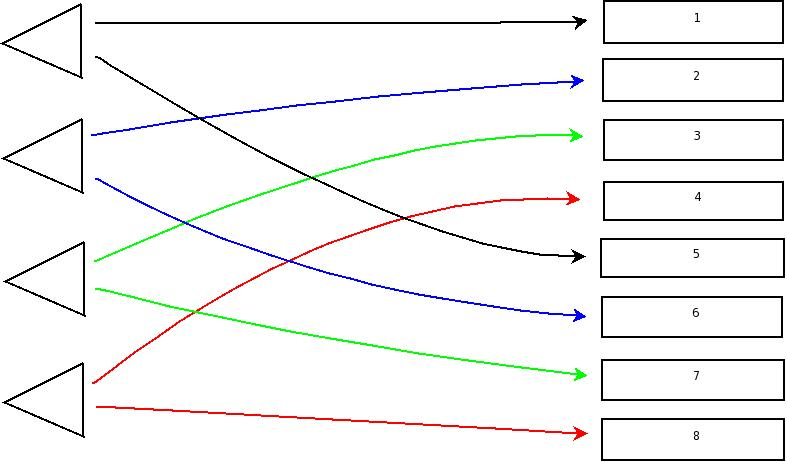
\includegraphics[width=4in]{vegas-quad-beam.jpg}
%\end{latexonly}
%\begin{htmlonly}
%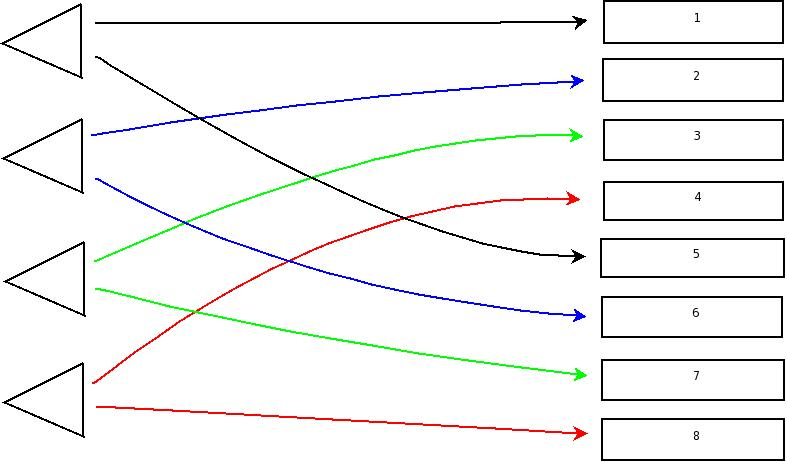
\includegraphics{vegas-quad-beam.jpg}
%\end{htmlonly}
%\end{center}
%\caption[KFPA Four Beams to VEGAS Mapping.]{A graphic demonstration of
%how KFPA four beam mode can be routed to the VEGAS banks.
%Each beam can be routed to 1 or 2 different VEGAS banks. }
%\label{fig:vegasquad}
%\end{figure}

%\begin{figure}[h!]
%\begin{center}
%\begin{latexonly}
%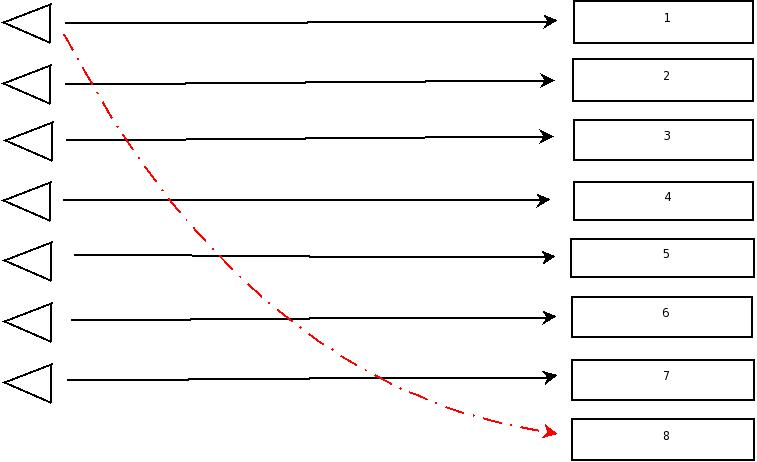
\includegraphics[width=4in]{vegas-seven-beam.jpg}
%\end{latexonly}
%\begin{htmlonly}
%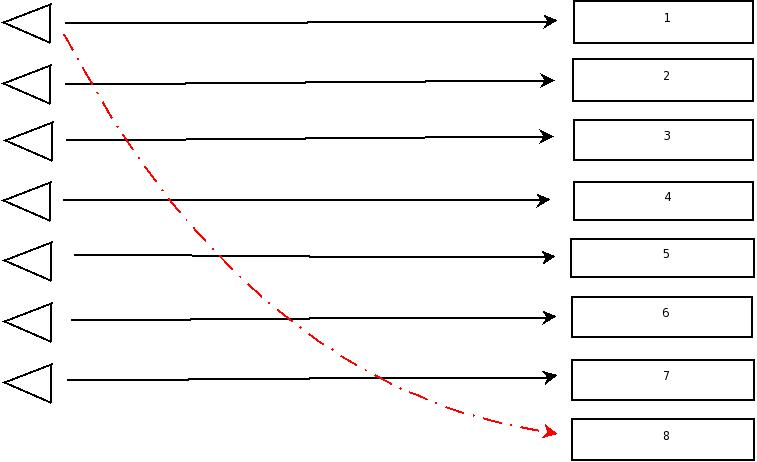
\includegraphics{vegas-seven-beam.jpg}
%\end{htmlonly}
%\end{center}
%\caption[KPFA seven beam to VEGAS Mapping.]{A graphic demonstration of
%how all seven beams of KFPA can be routed to the VEGAS banks.
%The routing of a second spectral window from beam 1 to bank
%H (7+1 mode of the KFPA) is optional.}
%\label{fig:vegasseven}
%\end{figure}










%\begin{table}[!h]
%\begin{footnotesize}
%\begin{center}
%\caption[Minimum recommended switching periods for VEGAS pointed
%observations without doppler tracking]
%{Minimum recommended switching periods (in seconds) for VEGAS pointed observations
%without doppler tracking.
%\label{tab:blanking_nodop}}
%\vspace{2.5mm}
%\begin{tabular}{ccccc}
%\toprule
%\multicolumn{1}{c}{\bf Mode} & \multicolumn{2}{c}{\bf{\Gls{tpower}}} & \multicolumn{2}{c}{{\bf\Gls{fsw}}$^e$} \\
%\cmidrule(lr){2-3}\cmidrule(lr){4-5}
% & {\tt tp\_nocal}$^a$ & {\tt tp}$^b$ & {\tt sp\_nocal}$^c$ & {\tt sp}$^d$ \\
%\midrule
%1  &  0.0005 &  0.0100 &  0.4000 &  0.4000 \\ 
%2  &  0.0014 &  0.0280 &  0.4000 &  0.4000 \\ 
%3  &  0.0020 &  0.0400 &  0.4000 &  0.4000 \\ 
%4  &  0.0100 &  0.0280 &  0.4000 &  0.4000 \\ 
%5  &  0.0199 &  0.0559 &  0.4000 &  0.4000 \\ 
%6  &  0.0301 &  0.1118 &  0.4000 &  0.4318 \\ 
%7  &  0.0102 &  0.0524 &  0.4000 &  0.4000 \\ 
%8  &  0.0203 &  0.1049 &  0.4000 &  0.4249 \\ 
%9  &  0.0301 &  0.2097 &  0.4000 &  0.5297 \\ 
%10 &  0.0056 &  0.2237 &  0.4000 &  0.5437 \\ 
%11 &  0.0112 &  0.4474 &  0.4474 &  0.8948 \\ 
%12 &  0.0280 &  0.8948 &  0.8948 &  1.7896 \\ 
%13 &  0.0447 &  1.7896 &  1.7896 &  3.5791 \\ 
%14 &  0.0671 &  3.5791 &  3.5791 &  7.1583 \\ 
%15 &  0.0056 &  0.4474 &  0.4474 &  0.8948 \\ 
%16 &  0.0112 &  0.8948 &  0.8948 &  1.7896 \\ 
%17 &  0.0336 &  1.7896 &  1.7896 &  3.5791 \\ 
%18 &  0.0447 &  3.5791 &  3.5791 &  7.1583 \\ 
%19 &  0.0895 &  7.1583 &  7.1583 & 14.3166 \\ 
%20 &  0.0051 &  0.0280 &  0.4000 &  0.4000 \\ 
%21 &  0.0101 &  0.0559 &  0.4000 &  0.4000 \\ 
%22 &  0.0301 &  0.1118 &  0.4000 &  0.4318 \\ 
%23 &  0.0405 &  0.2237 &  0.4000 &  0.5437 \\ 
%24 &  0.0755 &  0.4474 &  0.4474 &  0.8948 \\ 
%25 &  0.0070 &  0.0388 &  0.4000 &  0.4000 \\ 
%26 &  0.0141 &  0.0777 &  0.4000 &  0.4000 \\ 
%27 &  0.0398 &  0.1553 &  0.4000 &  0.4753 \\ 
%28 &  0.0544 &  0.3107 &  0.4000 &  0.6307 \\ 
%29 &  0.1010 &  0.6214 &  0.6214 &  1.2428 \\ 
%\bottomrule
%\end{tabular}
%\end{center}
%\end{footnotesize}
%\end{table}
%\begin{footnotesize}
%\begin{itemize}[itemsep=0pt]
%\item[$^a$] Recommended minimum switching period ({\tt swper}) for \gls{tpower}
%observations without the \gls{noiseDiode} ({\tt swtype='tp\_nocal'}) and without
%Doppler tracking. This value is equivalent to the hardware exposure value for VEGAS.
%\item[$^b$] Recommmended minimum switching period ({\tt swper}) for \gls{tpower}
%observations with the \gls{noiseDiode} ({\tt swtype='tp'}) and without
%Doppler tracking. This switching period will result in less than 10\% of the data
%being blanked.
%\item[$^c$] Recommended minimum switching period ({\tt swper}) for \gls{fsw}
%observations without the \gls{noiseDiode} ({\tt swtype='sp\_nocal'}) and without
%Doppler tracking. This switching period will result in less than 10\% of the data
%being blanked.
%\item[$^d$] Recommended minimum switching period ({\tt swper}) for \gls{fsw}
%observations with the \gls{noiseDiode} ({\tt swtype='sp'}) and without Doppler
%tracking. This switching period will result in less than 10\% of the data being
%blanked.
%\item[$^e$] Due to \gls{LOone} settling time when \gls{fsw}, all switch periods
%must be $>$0.4 seconds.
%\end{itemize}
%\end{footnotesize}


% \begin{table}[!h]
% \begin{small}
% \begin{center}
% \caption[Minimum recommended switching periods for VEGAS mapping
% observations with doppler tracking]
% {Minimum recommended switching periods (in seconds) for VEGAS mapping observations
% with doppler tracking.
% \label{tab:blanking_dop_mapping}}
% \begin{tabular}{ccccc}
% \toprule
% \multicolumn{1}{c}{\bf Mode} & \multicolumn{2}{c}{\bf{\Gls{tpower}}} & \multicolumn{2}{c}{{\bf\Gls{fsw}}$^e$} \\
% \cmidrule(lr){2-3}\cmidrule(lr){4-5}
%  & {\tt tp\_nocal}$^a$ & {\tt tp}$^b$ & {\tt sp\_nocal}$^c$ & {\tt sp}$^d$ \\
% \midrule
% 1  &  0.0010 &  0.0100 &  0.4000 &  0.4000 \\ 
% 2  &  0.0028 &  0.0280 &  0.4000 &  0.4000 \\ 
% 3  &  0.0040 &  0.0400 &  0.4000 &  0.4000 \\ 
% 4  &  0.0114 &  0.0280 &  0.4000 &  0.4000 \\ 
% 5  &  0.0227 &  0.0559 &  0.4000 &  0.4000 \\ 
% 6  &  0.0357 &  0.1118 &  0.7600 &  1.5200 \\ 
% 7  &  0.0128 &  0.0524 &  0.4000 &  0.4000 \\ 
% 8  &  0.0256 &  0.1049 &  0.7600 &  1.5200 \\ 
% 9  &  0.0406 &  0.2097 &  0.7600 &  1.5200 \\ 
% 10 &  0.0168 &  0.2237 &  0.7600 &  1.5200 \\ 
% 11 &  0.0336 &  0.4474 &  0.7600 &  1.5200 \\ 
% 12 &  0.0727 &  0.8948 &  0.8948 &  1.7896 \\ 
% 13 &  0.1342 &  1.7896 &  1.7896 &  3.5791 \\ 
% 14 &  0.2461 &  3.5791 &  3.5791 &  7.1583 \\ 
% 15 &  0.0280 &  0.4474 &  0.7600 &  1.5200 \\ 
% 16 &  0.0559 &  0.8948 &  0.8948 &  1.7896 \\ 
% 17 &  0.1230 &  1.7896 &  1.7896 &  3.5791 \\ 
% 18 &  0.2237 &  3.5791 &  3.5791 &  7.1583 \\ 
% 19 &  0.4474 &  7.5383 &  7.1583 & 14.3166 \\ 
% 20 &  0.0065 &  0.0280 &  0.4000 &  0.4000 \\ 
% 21 &  0.0129 &  0.0559 &  0.4000 &  0.4000 \\ 
% 22 &  0.0357 &  0.1118 &  0.7600 &  1.5200 \\ 
% 23 &  0.0517 &  0.2237 &  0.7600 &  1.5200 \\ 
% 24 &  0.0979 &  0.4474 &  0.7600 &  1.5200 \\ 
% 25 &  0.0090 &  0.0388 &  0.4000 &  0.4000 \\ 
% 26 &  0.0180 &  0.0777 &  0.7600 &  1.5200 \\ 
% 27 &  0.0476 &  0.1553 &  0.7600 &  1.5200 \\ 
% 28 &  0.0699 &  0.3107 &  0.7600 &  1.5200 \\ 
% 29 &  0.1320 &  0.6214 &  0.7600 &  1.5200 \\ 
% \bottomrule
% \end{tabular}
% \end{center}
% \end{small}
% \end{table}

% \begin{small}
% \begin{itemize}[itemsep=0pt]
% \item[$^a$] Recommended minimum switching period ({\tt swper}) for
% Doppler-tracked, \gls{tpower} \gls{OTF} maps with no \gls{noiseDiode}
% ({\tt swtype='tp\_nocal'}). These values will yield less than 10\% blanking overall
% and assume that the maps are sampled at twice Nyquist in the scanning direction and
% that there are four integrations per switching period.
% \item[$^b$] Recommmended minimum switching period ({\tt swper}) for
% Doppler-tracked, \gls{tpower} \gls{OTF} maps with the \gls{noiseDiode}
% ({\tt swtype='tp'}). These values will yield less than 10\% blanking
% overall and assume that the maps are sampled at twice Nyquist in the
% scanning direction and that there are four integrations per switching period.
% \item[$^c$] Recommended minimum switching period ({\tt swper}) for
% Doppler-tracked, \gls{fsw} observations with the \gls{noiseDiode}
% turned off ({\tt swtype='sp\_nocal'}). These values will yield less than 10\%
% blanking in the first state of the switching cycle as well as less
% than 10\% blanking overall.  This switching period will result in
% less than 10\% of your data being blanked. These values assume that
% the maps are sampled at twice Nyquist in the scanning direction and
% that there are four integrations per switching period.
% \item[$^d$] Recommended minimum switching period ({\tt swper}) for
% Doppler-tracked, \gls{fsw} observations with the \gls{noiseDiode}
% turned on ({\tt swtype='sp'}). These values will yield less than 10\%
% blanking in the first state of the switching cycle as well as less
% than 10\% blanking overall. These values assume that the maps are
% sampled at twice Nyquist in the scanning direction and that there are
% four integrations per switching period.
% \item[$^e$] Due to \gls{LOone} settling time when \gls{fsw}, all switch periods
% must be $>$0.4 seconds.
% \end{itemize}
% \end{small}

% \newpage


% \begin{table}[!h]
% \begin{center}
% \begin{footnotesize}
% \caption[Minimum recommended switching periods for VEGAS pointed observations with
% doppler tracking]
% {Minimum recommended switching periods (in seconds) for VEGAS pointed
% observations with doppler tracking.
% \label{tab:blanking_dop}}
% \begin{tabular}{c cc cc|cc cc}
% \toprule
% & \multicolumn{4}{c}{\Gls{tpower}} &  \multicolumn{4}{c}{\Gls{fsw}} \\
% \cmidrule(l{1cm}r{1cm}){2-5}\cmidrule(l{1cm}r{1cm}){6-9}
% & \multicolumn{2}{c}{\tt tp\_nocal} & \multicolumn{2}{c}{\tt tp} &
% \multicolumn{2}{c}{\tt sp\_nocal} & \multicolumn{2}{c}{\tt sp} \\
% \cmidrule(l{5mm}r{5mm}){2-3}\cmidrule(l{5mm}r{5mm}){4-5}
% \cmidrule(l{5mm}r{5mm}){6-7}\cmidrule(l{5mm}r{5mm}){8-9}
% {\bf Mode} & $\nu_{min}$ (GHz) & swper$^a$ (s) & $\nu_{min}$ (GHz) & swper$^b$ (s) &
%              $\nu_{min}$ (GHz) & swper$^c$ (s) & $\nu_{min}$ (GHz) & swper$^d$ (s) \\
% \hline

% 1 & 115.0 &  0.0005 & 115.0 &  0.0100 & 115.0 &  0.7600 & 115.0 &  1.5200 \\ 
% 2 & 115.0 &  0.0014 & 115.0 &  0.0280 & 115.0 &  0.7600 & 115.0 &  1.5200 \\ 
% 3 & 115.0 &  0.0020 & 115.0 &  0.0400 & 115.0 &  0.7600 & 115.0 &  1.5200 \\ 
% 4 & 115.0 &  0.0100 & 115.0 &  0.0280 & 115.0 &  0.7600 & 115.0 &  1.5200 \\ 
% 5 & 115.0 &  0.0199 & 115.0 &  0.0559 & 115.0 &  0.7600 & 115.0 &  1.5200 \\ 
% 6 & 115.0 &  0.0301 & 115.0 &  0.1118 & 115.0 &  0.7600 & 115.0 &  1.5200 \\ 
% 7 & 115.0 &  0.0102 & 115.0 &  0.0524 & 115.0 &  0.7600 & 115.0 &  1.5200 \\ 
% 8 & 115.0 &  0.0203 & 115.0 &  0.1049 & 115.0 &  0.7600 & 115.0 &  1.5200 \\ 
% 9 & 115.0 &  0.0301 & 115.0 &  0.2097 & 115.0 &  0.7600 &  59.6 &  1.5200 \\ 
% 10 & 115.0 &  0.0056 & 115.0 &  0.2237 & 115.0 &  0.7600 &  54.4 &  1.5200 \\ 
% 11 & 115.0 &  0.0112 &  33.1 &  0.4474 &  33.1 &  0.7600 &  16.5 &  1.5200 \\ 
% 12 & 115.0 &  0.0280 &   8.3 &  0.8948 &   8.3 &  0.8948 &   4.1 &  1.7896 \\ 
% 13 &  82.7 &  0.0447 &   2.1 &  1.7896 &   2.1 &  1.7896 &   1.0 &  3.5791 \\ 
% 14 &  27.6 &  0.0671 &   0.5 &  3.5791 &   0.5 &  3.5791 &   0.3 &  7.1583 \\ 
% 15 & 115.0 &  0.0056 &  33.1 &  0.4474 &  33.1 &  0.7600 &  16.5 &  1.5200 \\ 
% 16 & 115.0 &  0.0112 &   8.3 &  0.8948 &   8.3 &  0.8948 &   4.1 &  1.7896 \\ 
% 17 & 110.3 &  0.0336 &   2.1 &  1.7896 &   2.1 &  1.7896 &   1.0 &  3.5791 \\ 
% 18 &  41.3 &  0.0447 &   0.5 &  3.5791 &   0.5 &  3.5791 &   0.3 &  7.1583 \\ 
% 19 &  10.3 &  0.3800 &   0.1 &  7.5383 &   0.1 &  7.1583 &   0.1 & 14.3166 \\ 
% 20 & 115.0 &  0.0051 & 115.0 &  0.0280 & 115.0 &  0.7600 & 115.0 &  1.5200 \\ 
% 21 & 115.0 &  0.0101 & 115.0 &  0.0559 & 115.0 &  0.7600 & 115.0 &  1.5200 \\ 
% 22 & 115.0 &  0.0301 & 115.0 &  0.1118 & 115.0 &  0.7600 & 115.0 &  1.5200 \\ 
% 23 & 115.0 &  0.0405 & 115.0 &  0.2237 & 115.0 &  0.7600 &  54.4 &  1.5200 \\ 
% 24 & 115.0 &  0.0755 &  33.1 &  0.4474 &  33.1 &  0.7600 &  16.5 &  1.5200 \\ 
% 25 & 115.0 &  0.0070 & 115.0 &  0.0388 & 115.0 &  0.7600 & 115.0 &  1.5200 \\ 
% 26 & 115.0 &  0.0141 & 115.0 &  0.0777 & 115.0 &  0.7600 & 115.0 &  1.5200 \\ 
% 27 & 115.0 &  0.0398 & 115.0 &  0.1553 & 115.0 &  0.7600 &  89.7 &  1.5200 \\ 
% 28 & 115.0 &  0.0544 &  68.6 &  0.3107 &  68.6 &  0.7600 &  33.8 &  1.5200 \\ 
% 29 & 105.5 &  0.1010 &  17.1 &  0.6214 &  17.1 &  0.7600 &   8.6 &  1.5200 \\ 

% \bottomrule
% \end{tabular}

% \end{footnotesize}
% \end{center}
% \end{table}

% \begin{small}
% \begin{itemize}[itemsep=1pt]
% \item[$\nu_{min}$] The frequency above which you should use the minimum
% recommended switching period values in this table. Below this the values in
% Table~\ref{tab:blanking_nodop} are appropriate.
% \item[$^a$] Recommended minimum switching period for pointed, Doppler-tracked,
% \gls{tpower} observations without the \gls{noiseDiode} ({\tt swtype='tp\_nocal'}). These
% values will yield less than 10\% blanking overall.
% \item[$^b$] Recommended minimum switching period for pointed, Doppler-tracked,
% \gls{tpower} observations with the \gls{noiseDiode} ({\tt swtype='tp'}). These values will
% yield less than 10\% blanking overall.
% \item[$^c$] Recommended minimum switching period for pointed, Doppler-tracked,
% \gls{fsw} observations without the \gls{noiseDiode} diode ({\tt swtype='sp\_nocal'}). These
% values will yield less than 10\% blanking in the first state of the switching
% cycle as well as less than 10\% blanking overall.
% \item[$^d$] Recommended minimum switching period for pointed, Doppler-tracked,
% %\gls{fsw} observations with the \gls{noiseDiode} ({\tt swtype='sp'}). These values will
% %yield less than 10\% blanking in the first state of the switching cycle as well
% %as less than 10\% blanking overall.
% %\end{itemize}
% %\end{small}
% %herez
% %\newpage